%課題研究レジュメテンプレート ver. 1.2

\documentclass[uplatex]{jsarticle}
\usepackage[top=20mm,bottom=20mm,left=20mm,right=20mm]{geometry}
\usepackage[T1]{fontenc}
\usepackage{txfonts}
\usepackage{wrapfig}
\usepackage[expert,deluxe]{otf}
\usepackage[dvipdfmx,hiresbb]{graphicx}
\usepackage[dvipdfmx]{hyperref}
\usepackage{pxjahyper}
\usepackage{secdot}
\usepackage{here}

\makeatletter
  \renewcommand{\section}{%
    \if@slide\clearpage\fi
    \@startsection{section}{1}{\z@}%
    {\Cvs \@plus.5\Cdp \@minus.2\Cdp}% 前アキ
    {.5\Cvs \@plus.3\Cdp}% 後アキ
    %{\normalfont\Large\headfont\raggedright}}
    {\normalfont\raggedright}}

  \renewcommand{\subsection}{\@startsection{subsection}{2}{\z@}%
    {\Cvs \@plus.5\Cdp \@minus.2\Cdp}% 前アキ
    {.5\Cvs \@plus.3\Cdp}% 後アキ
    %{\normalfont\large\headfont}}
    {\normalfont}}

  \renewcommand{\subsubsection}{\@startsection{subsubsection}{3}{\z@}%
    {\Cvs \@plus.5\Cdp \@minus.2\Cdp}%
    {\z@}%
    %{\normalfont\normalsize\headfont}}
    {\normalfont}}
\makeatother
%ここから上を編集する必要はない.





\title{\vspace{-14mm}ルーブリック評価を利用したPBLにおける学習到達度の測定}
\author{PMコース 矢吹研究室 1342015 板倉 啓太}
\date{}%日付を入れる必要はない.
\pagestyle{empty}%ページ番号は振らない.
\begin{document}
\maketitle





\section{研究の背景}

近年,情報系の分野における実践的な教育方法として,PBLに対する注目度が高まっている\cite{PBL}\cite{PBL1}.PBLは,Project Based Learning(プロジェクト・ベースト・ラーニング)の略称であり,「プロジェクト型学習」や「問題解決型授業」などと言われる.PBLは欧米発祥の教育手法であり,日本では医歯薬学の分野など実習・演習が重視される分野において,以前から有効な教育手法として知られてきた.PBLが特にここ数年,情報系での分野の新しい教育手法として大きな注目を集め始めている.現在の社会では情報技術が多くの産業の基盤となり,情報技術 に関する高い技術力や活用力を有する人材がこれまで以上に強く求められるようになっている.その背景には,情報系分野における教育に対して,現在以上の実践性が必要だと考える強い問題意識の台頭である.こうした中で,高度な人材の育成に向けて,より実践的な教育を実現するための効果的な教育手法として,PBLが注目を集めているのである.

しかし実際のところ,PBLの実施方法に関する論文や書籍はまだ少ないため,PBLを実施している大学の多くは限られた情報の中で課題を設計・実施しているのが現状である.加えて,現在のPBLの教育方法は全ての参加者に対して,有効的な教育ツールではなく,常に改善が求められている.また,PBLを取り入れた授業の学生個人に対する評価は,PBLがグループ作業を基本としているため,個人が実践し,学んだ内容が知識として身に付いているかという評価をすることが困難である.そこで行動特性の定量的な評価をするために,ルーブリック評価という手法がある\cite{ルーブリック評価}.行動特性とは,成果に結びつき,安定的に継続して発揮されている能力である.ルーブリック は,学習到達度を示す評価基準を観点と尺度からなる表として示したものである.

これらの点を踏まえ,ルーブリック評価の手法を用いて,アンケート表を作成し,個人の学習到達状況を調査し,今後の改善案を模索し提案する.




\section{研究の目的}

本研究では,今回は,プロジェクトマネジメント学科のソフトウェアコースのPM実験を受講した学生を対象に,ルーブリック評価の手法を用いて4段階評価でアンケートを作成し,学習到達度を調査する.4段階評価での学習到達度の定義は下記に記す.調査した結果を基に,今後のPM実験における改善案を考察する.

\begin{itemize}

\item 知識が全く身に付いていない「評価1」
\item 実験をする上で,どの手法を使えば良いか理解している「評価2」
\item 必要な知識が身に付いており,一人でも行える「評価3」
\item 必要な知識が身に付き,問題が発生した際でも対応し,応用ができる「評価4」

\end{itemize}







\section{プロジェクトマネジメントとの関連}

PBLはプロジェクト型学習とも呼ばれ,プロジェクトを通しての課題の解決を目標にした教育手法である.これは,プロジェクトマネジメントの知識エリアにおいては主にプロジェクト統合マネジメントに該当する.加えて,プロジェクト・コミュニケーション・マネジメントやプロジェクト・スコープ・マネジメントにも該当する.








\section{研究の方法}

以下の順に研究を進める.

\begin{enumerate}
\item ソフトウェアコースのPM実験を受講した学生に対し,4段階評価でのアンケート調査をする.
\item ルーブリック評価の手法を用いて,アンケート項目ごとの定義を段階別に設定する.
\item アンケート結果を基に,PM実験を終えた学生の学習到達度をグラフ化し,今後の改善案を考察する.

\end{enumerate}








\section{現在の進捗状況}

上記の手順で,PM実験のソフトウェアコースを学習し終えた一部の学生からアンケート調査を行った.下記にアンケート結果を記す.最終的な成果物の提出期限には間に合っていたものの,プロジェクトを進行していく上で,計画の遅延に対するリスクの測定・対応が不足している事が判明した.またプレゼンテーションの際,図表やグラフを用いた表現が少ないという点も判明した.これらの結果から,発表資料にグラフを用いて,聴衆に対する理解度を向上させる必要がある.また,計画の遅延に対して,リスク登録簿を作成することで発生したリスクの対応がしやすくなり,遅延が改善されるではないかと考察する.




\section{今後の計画}

以下のように研究を進める計画である.

\begin{enumerate}
\item 今回作成したアンケート項目では,PM実験での学習到達度を的確に測定出来ていないため,アンケート項目の追加・修正を行う.
\item 調査対象である学生の回答者数を増やす.
\item 論文の執筆を行う.
\end{enumerate}


\begin{center}
  \begin{figure}[H]
    \begin{tabular}{cc}
      %---- 最初の図 ---------------------------
      \begin{minipage}[t]{0.45\hsize}
        \centering
        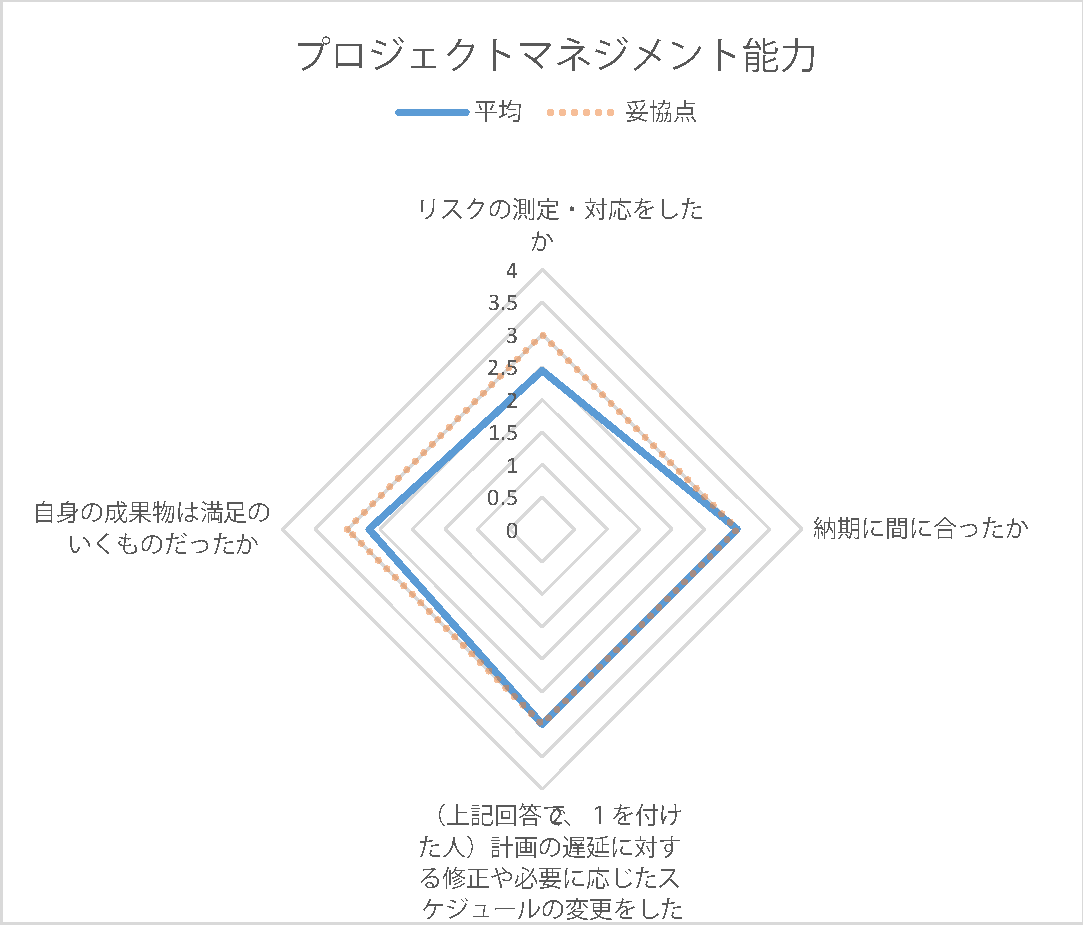
\includegraphics[keepaspectratio, scale=0.4]{g1.pdf}
        \caption{アンケート項目1}
        \label{ラベル1}
      \end{minipage} &
      %---- 2番目の図 --------------------------
      \begin{minipage}[t]{0.60\hsize}
        \centering
        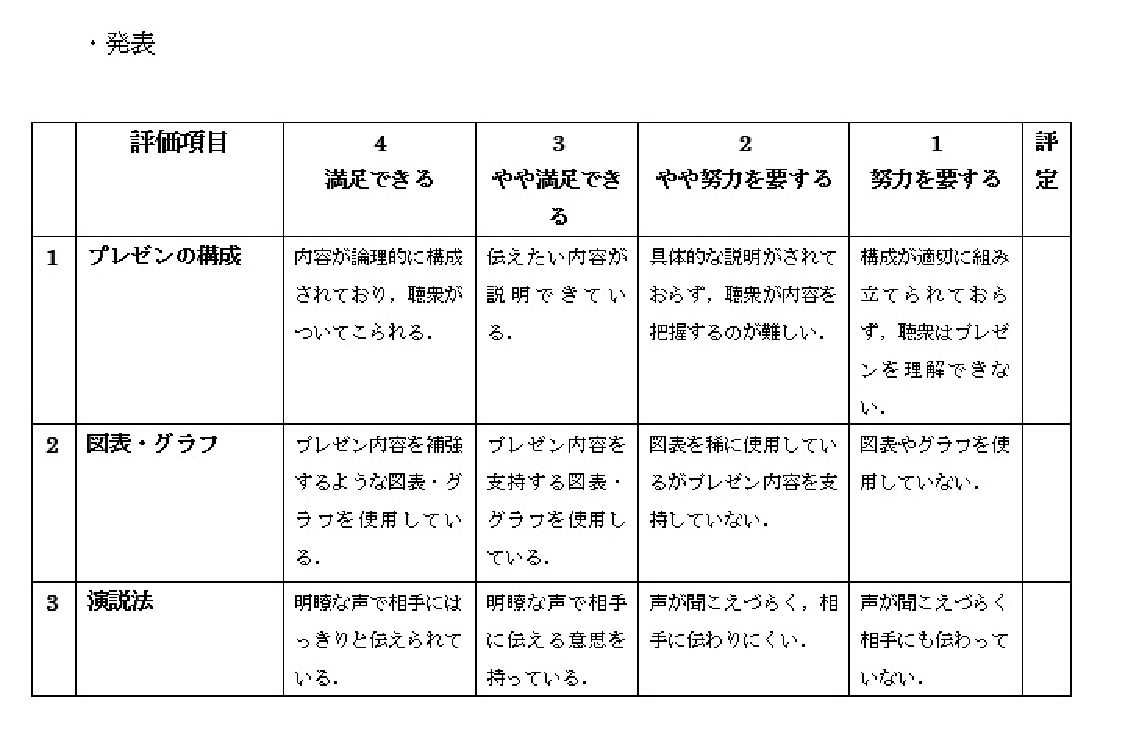
\includegraphics[keepaspectratio, scale=0.4]{g2.pdf}
        \caption{アンケート項目2}
        \label{ラベル2}
      \end{minipage}
      %---- 図はここまで ----------------------
    \end{tabular}
  \end{figure}
\end{center}


\bibliographystyle{junsrt}
\bibliography{biblio}%「biblio.bib」というファイルが必要.

\end{document}
